\documentclass[tikz,border=5pt]{standalone}
\usepackage{verbatim}
\usetikzlibrary{shadings,intersections}

\begin{document}
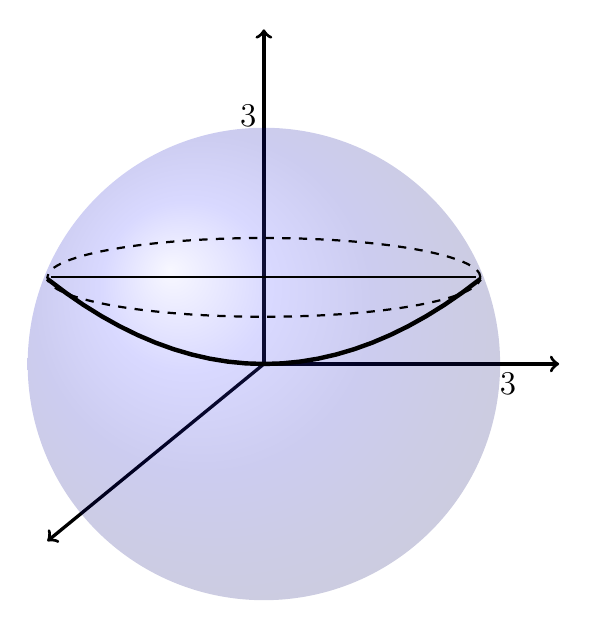
\begin{tikzpicture}

% \coordinate (O) at (0,0);
  \draw [very thick, ->] (0, 0) -- (3.75, 0);
  \draw [very thick, ->] (0, 0) -- (-2.75, -2.25);
  \draw [very thick, ->] (0, 0) -- (0, 4.25);

  \shade[ball color = blue, opacity = 0.2] (0, 0) circle (3);
 \draw [ultra thick,  domain=-2.75:2.75, variable=\x] plot ({\x},{\x*\x /7});
   
 % \draw [ultra thick, black!30!green] (0, 0) -- (2, 2) ;
 
 \draw [ thick, dashed] (0, 1.1) ellipse (2.75 and .5);

  \draw [thick] (-2.7, 1.1) -- (2.7, 1.1) ;
  \draw (-.2, 3.15) node {\large 3};
  \draw (3.1, -.25) node {\large 3};


\end{tikzpicture}
\end{document}
